The discovery of the Higgs boson completed the Standard Model in 2012 and confirmed the Higgs mechanism for the electroweak symmetry breaking and mass generation. Beyond this, we are able to measure its couplings to other particles as well as its decay modes.

\begin{figure}[pht]
  \centering
  \subfloat[Higgs coupling constants vs particle mass, Taken from~\cite{LHC_Higgs_handbook}]{
    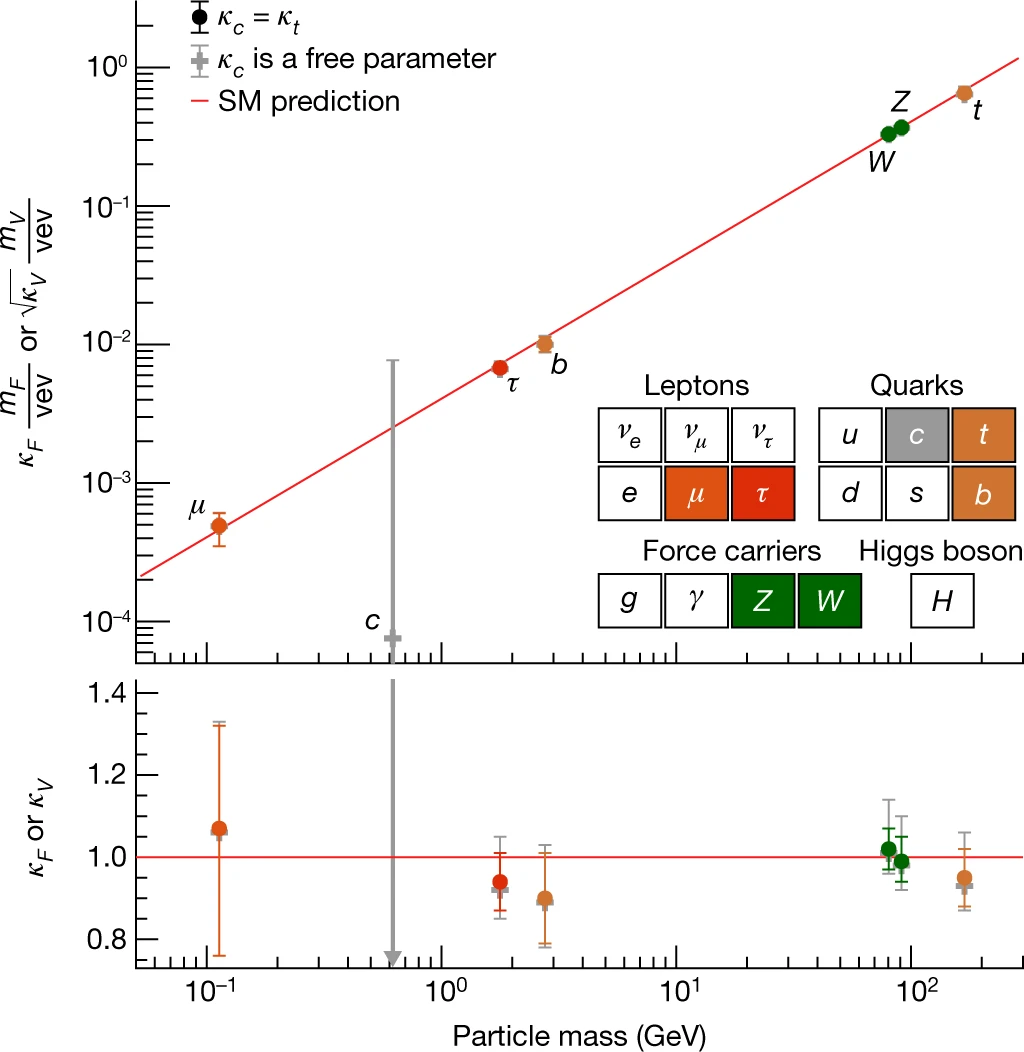
\includegraphics[width=0.45\textwidth]{figures/theory/theory_coupling_strengths.png}\label{fig:coupling_vs_mass}
  }\hspace{0.01\textwidth}
  \subfloat[Higgs boson branching ratios vs mass, Taken from~\cite{ATLAS_Open_Data}]{
    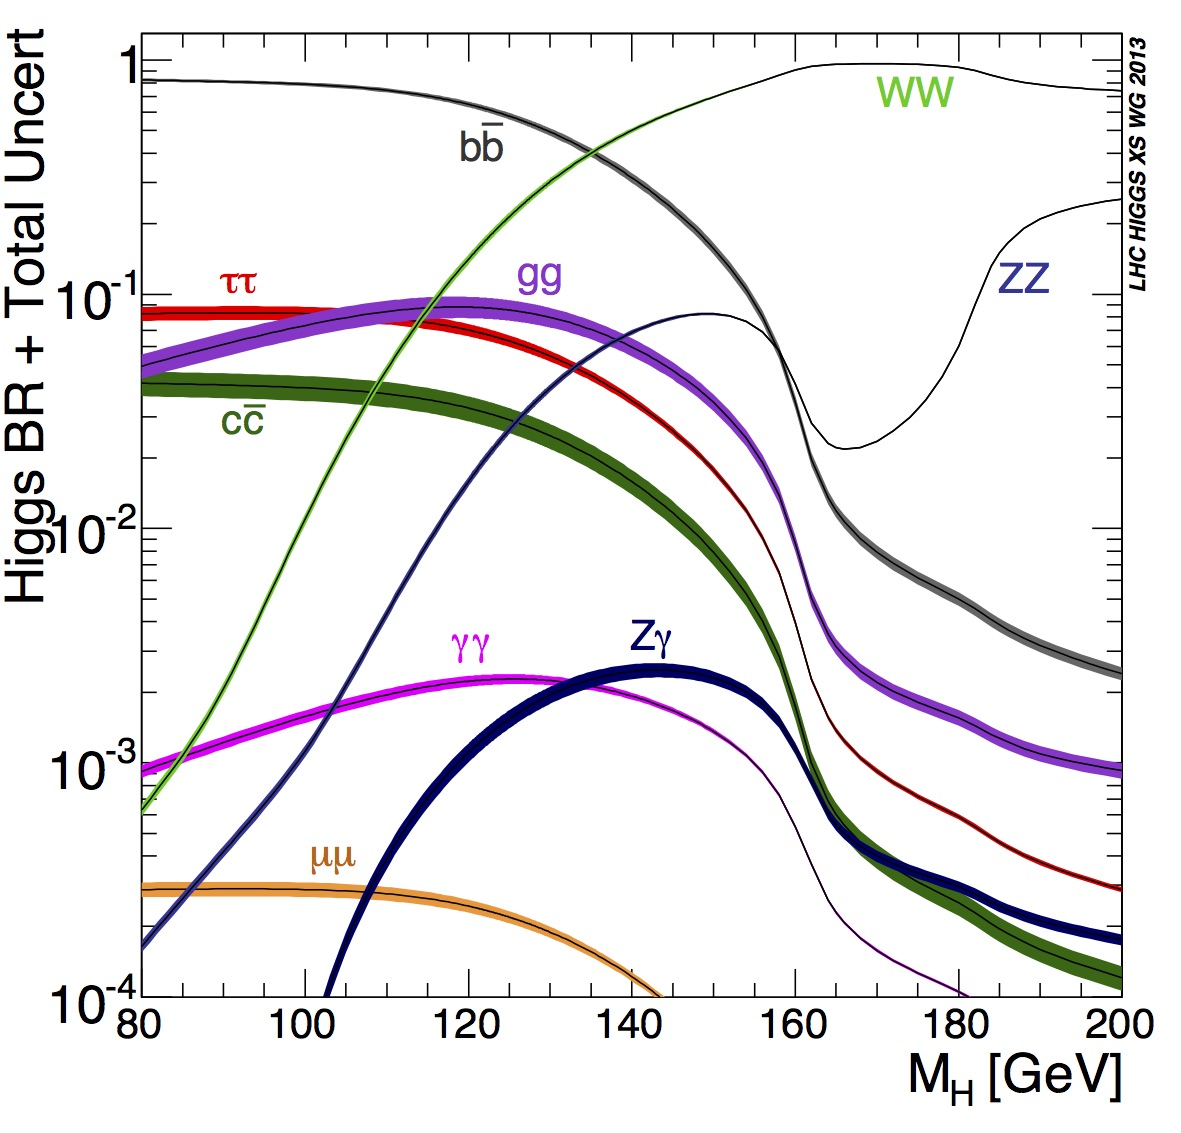
\includegraphics[width=0.45\textwidth]{figures/theory/theory_higgs_br_vs_mass.jpg}\label{fig:Higgs_BR_mass_range}
  }
\end{figure}

In the SM, the Higgs boson couples to fermions with strength proportional to their mass ($g_{Hff} = \frac{m_{f}}{v}$) and to vector bosons with a strength proportional to the square of their mass ($g_{HVV} = \frac{2m_{V}^{2}}{v}$). Figure~\ref{fig:coupling_vs_mass} shows the reduced Higgs coupling constants as a function of particle mass as measured by ATLAS\@. The results confirm the expected mass dependence of the couplings where heavier particles couple more strongly to the Higgs boson. Couplings to all vector bosons and third-generation fermions have been measured, while efforts to measure couplings to second-generation fermions are ongoing.

These coupling indicate that the Higgs boson tends to decay into the heaviest particles that are kinematically allowed. Figure~\ref{fig:Higgs_BR_mass_range} illustrates the branching ratios of the Higgs boson as a function of its mass. Since the Higgs boson coupling to vector bosons scales as $m_{V}^{2}$, decays to vector boson pairs become dominant at high Higgs boson masses, where the Higgs boson is sufficiently heavy to decay into two on-shell bosons. However, the Higgs boson we measure has mass $m_{H} = 125$ GeV, so the dominant decay channel is H $\rightarrow b\bar{b}$, since the bottom quark is the heaviest fermion accessible at this mass. Vector boson decays are suppressed because at least one of the bosons must be off-shell. 

The sub-dominant decay is $H \rightarrow WW^{*}$, followed by $H \rightarrow gg$. While $H \rightarrow gg$ has the third highest branching ratio, it has yet to be measured due to the complexities of having a two $g$ final state. Following this, the next most common decay modes are $H \rightarrow \tau^{+}\tau^{-}$, $H \rightarrow ZZ^{*}$, and $H \rightarrow \gamma\gamma$. The predicted branching ratios for a Higgs boson of mass $m_{H} = 125$ GeV is listed in Table~\ref{tab:BRs}.

\begin{table}[h]
  \centering
  \begin{tabular}{l|c}
    \hline
    Decay Channel & Branching Ratio \\
    \hline
    $H \rightarrow b\bar{b}$ & $58.2^{+1.2}_{-1.3}$~\% \\
    $H \rightarrow W^{\pm}W^{*\mp}$ & $21.4^{+1.6}_{-1.5}~\%$ \\
    $H \rightarrow gg$ & $8.2^{+5.1}_{-5.1}~\%$ \\
    $H \rightarrow \tau^{+}\tau^{-}$ & $6.3^{+1.7}_{-1.7}~\%$ \\
    $H \rightarrow ZZ^{*}$ & $2.6^{+1.6}_{-1.5}~\%$ \\
    $H \rightarrow \gamma\gamma$ & $0.23^{+2.1}_{-2.1}~\%$ \\
    \hline
  \end{tabular}
  \caption{Predicted branching ratios for the Higgs boson decay channels at $m_{H} = 125$ GeV, taken from~\cite{LHC_Higgs_handbook}.}\label{tab:BRs}
\end{table}

Among these, the $H \rightarrow WW^{*}$ channel is of particular interest for this thesis. Despite being being the sub-dominant channel, it still maintains a high branching ratio of approximately 21\% providing a substantial number of events. Furthermore, the leptonic decay $WW^{*} \rightarrow \ell\nu\ell\nu$ provides a clean experimental signature in the ATLAS detector due to the excellent lepton identification and reconstruction. This makes an ideal channel for precision studies, and forms the basis of this thesis.

To study this decay channel, we must first produce Higgs bosons which will be discussed in the following Section.
